% -*- mode: LaTeX; coding: utf-8; -*-

% Testaa, onko tämä gradu vai seminaari (purkkaviritys)
\ifdefined\seminaari
\relax
\else
\chapter{Dynaamiset WWW-teknologiat}
\fi

\section{Yleistä}

Internet on aina ollut ja tulee aina olemaan vihamielinen paikka, jossa sivustolla vierailevan motiiveja sivustoa ja palvelua kohtaan on mahdotonta ennustaa. Tästä syystä 
useimmat kehittäjät ja ylläpitäjät ovat noudattaneet periaatetta, että keneenkään ei voi täysin luottaa. Sivustojen ja palveluiden kehittyessä entistä monimutkaisemmiksi,
on tämän ns. luottamattomuusperiaatteen noudattaminen noussut entistä
tärkeämmäksi.

Webin teknisen monimutkaistumisen taustalla on dynaamisuuden
lisääntyminen. Paljon sellaisia tehtäviä, jotka aiemmin olivat
palvelimen vastuulla, on siirretty käyttäjän selaimessa
suoritettavaksi. Lisäksi WWW-sivujen sisältö ei ole enää staattista,
vaan uutta sisältöä voidaan ladata sivulle käyttäen useitakin eri
teknologioita. Näistä dynaamisista WWW-teknologioista käytetään
usein nimitystä \emph{Web 2.0}.

Tämän \ifdefined\seminaari seminaariraportin \else luvun \fi tarkoitus
onkin lyhyesti esitellä tärkeimmät dynaamiset WWW-teknologiat, ja
tuoda esille merkittävimmät riskit, joita huonosti toteutetut
sovellukset voivat aiheuttaa.

\section {AJAX}

Jos jokin dynaamisista WWW-teknologiosta halutaan nostaa kehitystä
eniten eteenpäin vieväksi voimaksi, niin vahvin ehdokas tähän on AJAX.
Asynchronous JavaScript and XML (lyh. AJAX) itsessään ei ole mikään
yksi tietty teknologia, vaan se on usean eri teknologian yhdistelmä,
joita käyttämällä WWW-sivut pystytään muuttamaan nopeasti reagoiviksi
ja käyttökokemukseltaan muistuttamaan perinteisiä työpöytäsovelluksia
\cite{AJAX}. AJAX koostuu seuraavista teknologioista:

\begin{itemize}
\item HTML ja CSS rakentavat WWW-selaimella näytettävän sivun.
\item DOM mahdollistaa ajonaikaisen sisällön tuottamisen.
\item XML ja Extensible Stylesheet Language Transformation (lyh. XSLT)
  mahdollistavat eri komponenttien välisen tiedonsiirron.
\item JavaScript helpottaa eri komponenttien integroimisen sekä näiden
  ohjelmoimisen.
\item XMLHttpRequest (lyh. XHR) objekti helpottaa kommunikointia
  palvelinten kanssa \cite{WEB2b}.
\end{itemize}

Suurin AJAXin tuoma muutos perinteisiin WWW-sivuihin on mahdollisuus
päivittää sivun sisältöä asynkronisesti, ilman käyttäjän
vuorovaikutusta. Yksinkertaistettuna tämä tarkoittaa sitä, että sivun
sisällöstä pystytään päivittämään ainoastaan halutut osat käyttäen
XHR-kanavia. Aikaisemmin tällainen ei ole ollut mahdollista, sillä
vanhat WWW-sivut ovat toimineet pelkästään synkronisesti, jolloin
erillisiä kutsuja ei ole voitu tehdä. Tällöin koko sivu on täytynyt
päivittää kerralla. Tämä on hidastanut käyttökokemusta, sillä
päivityksen nopeus on riippunut siitä, kuinka nopeasti palvelin ja
selain ovat pystynyt käsittelemään koko sivun sisällön. XHR sisältää
kaikki perinteiset HTTP-metodit mukaanlukien GET, POST, HEAD ja
DELETE, joten sen avulla pystytään suorittamaan kaikki yleisimmät
käyttäjän toiminnot \cite{WEB2}. Kuvassa \ref{synkroninen} on esitetty
tilanne, jossa sama palvelu on toteutettu käyttäen synkronisia ja
asynkronisia kutsuja. Kuvasta voi havaita, että dynaamisuus, ns. Web
2.0, mahdollistaa useamman samanaikaisen kutsun tekemisen, jolloin
myös palvelun viiveet voidaan pitää lyhyinä.

\begin{figure}[htp]
\centering
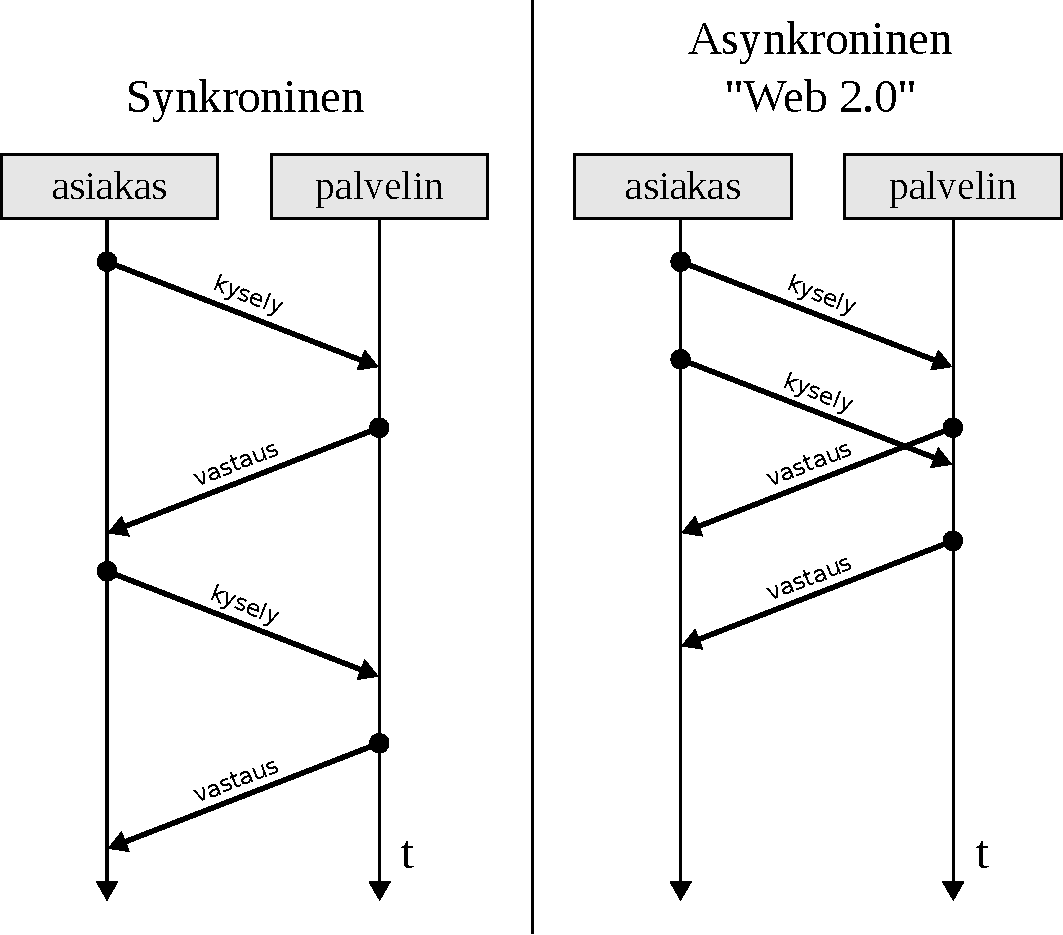
\includegraphics[width=12cm]{pics/synkroninen.pdf}
\caption{Synkroninen ja asynkroninen kommunikointi}
\label{synkroninen}
\end{figure}

AJAXiin kohdistuvat hyökkäykset eivät eroa suuresti vanhoista
murtautumismenetelmistä. Hyökkääjät pyrkivät edelleen hyödyntämään
syötteen puutteellista suodattamista, muokkaamaan ulostulevaa dataa,
murtamaan salauksia ja hankkimaan istuntonkohtaisia tietoja
esimerkiksi evästeitä varastamalla.

Hyökkääjien näkökulmasta AJAXin tekee erityisen kiinnostavaksi se,
että aiempaa suurempi osa WWW-palvelun käyttämästä laskennasta
suoritetaan käyttäjän WWW-selaimessa. Käyttäjän selaimeen, eli
ns. asiakaspuoleen, ei voi kuitenkaan koskaan luottaa, ja
JavaScriptien huolimaton käyttö avaa hyökkääjille lukuisia tapoja
murtautua palveluihin. Kyseessä on sinänsä pitkään tunnettu ongelma,
mutta kehittäjien kiinnostuksen siirtyessä AJAXiin ovat myös
hyökkääjät alkaneet kiinnittämään näihin enemmän huomiota \cite{AJAX}.
Monet käytetyistä AJAX-ympäristöistä sisältävät myös eriasteisia
tietoturvariskejä, joita hyökkääjät voivat hyödyntää \cite{JSH}.

\subsection{JavaScript}

JavaScript on Netscapen suunnittelema skriptikieli, joka tunnettiin
aluksi nimellä LiveScript. Sun Microsystemsin kehittämän
Java-ohjelmointikielen yleistyessä Netscape päättii muuttaa sen nimen
JavaScriptiksi, toivoen sen käytön yleistyvän Javan menestyksen
myötä. JavaScriptillä kirjoitetut skriptit sijoitetaan HTML:n
\texttt{<script>}-elementin sisään, josta voi olla myös viite
erilliseen lähdekooditiedostoon. JavaScript vaatii tuen selaimelta,
joka kuitenkin löytyy miltei jokaisesta WWW-selaimesta, mukaanlukien
yleisimmät mobiililaitteet.

JavaScript on tehokas työkalu, joka mahdollistaa monen muun toiminnon
ohella mm. dynaamisten WWW-sivujen tekemisen, viestien kirjoittamisen
selaimen tilariville, uusien ikkunoiden avaamisen ja interaktiivisten
lomakkeiden luomisen. Skriptien toiminta rajoittuu kuitenkin
WWW-selaimen toimintoihin, eikä sitä käyttäen voida esimerkiksi
kirjoittaa levylle ja levyn lukeminen rajoittuu pelkästään evästeisiin
\cite{JavaScript}. Näistä rajoituksista huolimatta JavaScript
mahdollistaa erittäin monipuolisten toimintojen toteuttamisen
WWW-ympäristössä.

Suurin osa WWW-sivuilla olevista skripteistä toimii siten, että ne
ladataan aluksi käyttäjän koneelle, jonka jälkeen ne suoritetaan
selaimessa. Skriptit sijaitsevat ja ne suoritetaan käyttäjien
koneilla, joten toimintaperiaatten selvittäminen ei ole hyökkääjälle
vaikeaa. Asiaa pystytään kuitenkin vaikeuttamaan muutamalla eri
tavalla. Näistä yksinkertaisin on \emph{obfuskointi}, jonka yhteydessä
koodista tehdään vaikeasti luettavaa. Aluksi poistetaan kommentointi
ja tyhjät rivivälit, seuraava askel on koodin muuttujien ja objektien
uudelleennimeäminen, jolloin hyökkääjän on vaikeampi päätellä näistä
skriptin toimintaperiaate. Nimet voidaan myös muuttaa esimerkiksi
binäärikoodiksi, mutta tämän haittapuolena on tiedoston koon
kasvaminen. Nämä keinot ovat kuitenkin vain hidasteita osaavalle
hyökkääjälle \cite{AJAX}. Palvelu tulisikin suunnitella siten, että
kaikki luottamuksellisen tiedon käsittely ja käyttäjän syötteen
tarkistukset suoritettaisiin WWW-palvelimella. Tällöin käyttäjän
selaimessa suoritettaisiin ainoastaan sellainen laskenta, joissa
käsitellään käyttäjää itseään koskevaa dataa.

Koneelle ladatut skriptit ajetaan oletuksena hyvin rajatussa tilassa,
jossa niillä on pääsy vain kyseistä sivun sisältämään dataan tai
siihen hyvin läheisesti kuuluviin dokumentteihin. JavaScript noudattaa
myös \ifdefined\seminaari \relax \else edellisessä luvussa esitettyä
\fi \emph{saman alkuperän} periaatetta, joka estää skriptien
suorittamisen muista In\-ter\-net-do\-mai\-nis\-ta kuin siitä, josta skripti on
ladattu. Näin vaikeutetaan hyökkäyksen tekemistä käyttäen
toiselta sivulta ladattua haitallista skriptiä, jonka avulla
voitaisiin esimerkiksi varastaa evästeitä ja urkkia näppäimistön
painallukset.  Aikaisemmin selaimet ovat sallineet joitain poikkeuksia
tähän periaatteeseen, mutta tietoturvasyistä nämä on kuitenkin
poistettu.

Liian tiukat tietoturvasäännöt eivät kuitenkaan toimi nykyaikaisten\\
WWW-palveluiden kanssa, ja tästä syystä \emph{saman alkuperän}
periaatetta on mahdollista löysentää. Esimerkiksi ulkoiset linkit,
jotka osoittavat toisella sivustolla olevaan skriptiin, ohittavat
\emph{saman alkuperän}, sillä vaikka itse skripti sijaitsee toisella
palvelimella niin se lasketaan kuuluvan siihen sivuun, jossa viittaus
lähdekooditiodostoon on.  Näin kutsutulla skriptillä on pääsy
sellaisiin evästeisiin ja tiedostoihin, joihin sillä ei välttämättä
tarvitsisi olla oikeuksia. Sivustojen ja palveluiden käyttäessä
resursseja entistä useammasta lähteestä eri palvelimista, voi tämä
aiheuttaa riskitilanteita, jos jonkin lähteen tietoturva on
vaarantunut \cite{AJAX}.

\subsection{AJAXiin liittyvät tietoturvariskit}

Koska AJAXin toiminta perustuu hyvin pitkälti JavaScriptin varaan,
niin on itsestään selvää, että hyökkääjät pyrkivät väärinkäyttämään
käyttäjän antamaa luottamusta JavaScriptin avulla.  Asiaa ei auta se,
että suurin osa sivustoista on jollakin asteella alttiina
XSS-hyök\-käyk\-sil\-le \cite{WEB2c} johtuen huonosti toteutetusta syötteen
suodatuksesta. Asetettuja suodatuksia pystytään myös kiertämään
käyttäen esimerkiksi kuvalinkkejä ja erilaisia HTML-elementtejä,
joiden avulla ajettava skripti voidaan hukuttaa muun syötteen
joukkoon. Juuri tästä syystä pelkästään tiettyjen merkkijonojen
suodattaminen ei takaa suojaa JavaScript-pohjaisilta
hyökkäyksiltä. Tehokkain ja yksinkertaisin keino onkin poistaa kaikki
HTML-e\-le\-ment\-tei\-hin kuuluvat merkit, jolloin esimerkiksi \texttt{<}-merkistä tulee
\texttt{\&lt;} ja \texttt{>}-merkistä \texttt{\&gt;}. Monet ympäristöt
mahdollistavat myös suoraan HTML-e\-le\-ment\-ti\-en poistamisen käyttäjien
jättämistä viesteistä \cite{AJAX}. Tälloin esimerkiksi WWW-foorumeilla
toisten käyttäjien lähettämistä viesteistä saadaan poistettua
mm. niiden sisältämä JavaScript-ohjelmakoodi.

\subsubsection{Evästeiden kaappaaminen}

Kasvaneella JavaScriptin käytöllä on suora vaikutus myös
XSS-hyök\-käys\-ten yleistymiseen. JavaScriptillä pääsee helposti
evästeisiin käsiksi käyttäen \emph{document.cookie}-oliota. Vaikka sen
käyttö onkin rajoitettu ainoastaan sen Internet-domainin evästeeseen,
josta kutsu on tehty, voidaan tämä rajoitus ohittaa melko
helposti. Hyökkääjälle riittää, että käyttäjä vierailee esimerkiksi
sellaisessa foorumissa tai blogissa, joissa käyttäjien viesteissä
sallitaan XHTML:n käyttö. Tämä mahdollistaa haitallisten skriptien
lähettämisen sivustolle ja pahaa aavistamaton käyttäjä, joka vierailee
tällä sivulla, joutuu tietämättään hyökkäyksen kohteeksi.

Yksi tapa suojautua evästeiden varastamiselta on käyttää
HTTP-only~-evästeitä, jolloin asiakaspuolen evästeitä ei pystytä
lukemaan. Näiden evästeiden tukeminen on kuitenkin selainkohtaista,
joten tämä ratkaisu ei aina välttämättä ole mahdollista
toteuttaa. XSS-hyök\-käyk\-set eivät myöskään rajoitu pelkästään
evästeiden varastamiseen, ja yhtä helposti hyökkääjä voi esimerkiksi
luoda skriptin, joka lukee näppäimistön painallukset ja lähettää ne
haluttuun osoitteeseen. HTTP-only evästeiden käyttö ei myöskään täysin
suojaa evästeitä, jos käytetään XHR-kutsuja. Tällöin hyökkääjän on
mahdollista lukea suoraan otsaketiedoista asetettuja arvoja.

Jotkut XHR-objekteihin liittyvät haavoittuvuudet ovat myös niin
syvällä XHMLHttpRequest-objekteissa, että kaikki nykyisin käytössä
olevat toteutukset ovat niille jossakin määrin alttiina. Kaapattujen
XHR-objektien tunnistaminen ei myöskään vielä ole mahdollista
\cite{AJAX}. Näistä syistä johtuen AJAX tarjoaa nyt ja tulevaisuudessa
hyökkääjille monia mahdollisuuksia murtaa asetettuja suojauksia.

\subsubsection{JSON}

Yksi yleisimmistä AJAXissa käytetyistä dataformaateista on JavaScript
Object Notationt (lyh. JSON). Se on ohjelmointikielestä riippumaton ja
laajasti tuettu WWW-palvelimella käytetyissä työkaluissa. Se on
rakenteeltaan hyvin kevyt, ja se koostuu kahdesta eri tietotyypistä:
objekteista ja taulukoista \cite{JSON}.

Formaatin heikkous piilee siinä, että taulukko itsessään on
kelvollinen JavaScript-syöte, jonka sisältö on mahdollista kaapata
\cite{AJAX}. Termi \emph{JavaScript Hijacking} kuvaa tällaista
tilannetta, jossa hyökkääjä ohittaa \emph{saman alkuperän} periaatteen
silloin, kun JavaScriptiä käytetään arkaluontoisen tiedon
lähettämiseen. Aiheesta tehdyn tutkimuksen \cite{JSH} mukaan lähes
jokainen käytetty AJAX-ympäristö on alttiina tällaisilla
hyökkäyksille. Käyttäen CSRF-hyökkäystä hyökkääjä pystyy
väärinkäyttämään JSON-for\-maat\-ti\-a, ja varastamaan sekä muokkaamaan
toiselle sivustolle lähetettäviä paketteja.  Tälläinen hyökkäys
voidaan toteuttaa useilla eri tavoilla mukaanlukien käyttäen
\texttt{script}-elementtiä, ja koska pyyntö tulee selaimen luottamasta
lähteestä, voidaan tällä tavoin ohittaa esimerkiksi SSL-suojaus
\cite{AJAX}. Suojautuminen tämän tyyppisiltä hyökkäyksiltä voidaan
toteuttaa monella eri tapaa, ja paras tulos saadaan yhdistelemällä
näitä. Koska CSRF-hyök\-käyk\-ses\-sä hyökkääjä joutuu toimimaan osittain
sokeasti, voidaan jokaiseen pyyntöön lisätä parametri, jota hyökkääjän
on vaikea arvata. Palvelin voidaan myös asettaa tarkistamaan HTTP
Referer -kenttä, jolla voidaan varmistaa, että pyyntö tulee sallitulta
taholta, vaikkakin Referer-kentän sisältö voidaan helposti
muuttaa. Toinen tapa on muokata vastaanottopäässä paketteja siten,
että hyökkääjä ei pysty ajamaan lähettämissään pyynnöissä skriptejä
\cite{JSH}

\section{Flash}

AJAXin ohella Macromedian suunnittelema ja nykyisin Adoben kehittämä
Flash on ollut yksi niistä merkittävistä tekniikoista, joita käyttämällä
YouTuben ja MySpacen kaltaiset menestyspalvelut ovat olleet
mahdollisia toteuttaa. Flashia käyttämällä kehittäjät ovat jo pitkään
pystyneet luomaan interaktiivista ja rikasta WWW-sisältöä
yksinkertaisista animaatioista aina monimutkaisiin peleihin ja
valikoihin asti. Suurin osa WWW-si\-vus\-toil\-la olevista mainoksista on
myös toteutettu käyttäen Flashia. Näistä syistä johtuen Flash Player
on yksi ohjelmistoalan de facto-alustoista, jonka käyttöaste yritys-
ja kuluttajapuolella on lähes 100 prosenttia \cite{Flash}.

Flashin käyttämä ActionScript-skriptikieli muistuttaa läheisesti
JavaScriptiä, ja sitä käyttäen on mahdollista mm. luoda uusia
TCP-yhteyksiä, ajaa JavaScriptiä selaimessa ja luoda sallittuihin
domaineihin HTTP-pyyn\-tö\-jä. Flashin käyttämä tietoturvamalli noudattaa
paljolti saman alkuperän periaatetta, jolla rajoitetaan eri
domaineissa sijaitsevien sovellusten kommunikointia. Domainien välinen
kommunikointi on kuitenkin sallittua, ja käytetty tietoturvapolitiikka
luetaan tähän tarkoitetusta XML-tiedostosta. Tämä XML-tiedosto
sijaitsee usein domainin juuressa, ja se sisältää ne domainit, jotka
saavat olla siihen yhteydessä.

Osa Flashiin kohdistuvista hyökkäyksistä pyrkiikin muokkaamaan
tietoturvapolitiikkatiedoston sisältöä siten, että kohde sallisi
yhteydet myös hyökkääjän käyttämästä osoitteesta. Tämä voidaan
toteuttaa esimerkiksi käyttämällä vihamielistä RSS-syötettä tai
luomalla tiedosto, joka sisältää uuden XML-tiedoston. Yksi tällaisista
hyökkäyksistä on Stefan Esserin luoma GIF-tiedosto, jonka kommenttiin
on piilotettu uusi tietoturvapolitiikka. Hyökkääjälle riittää, että
kohdekone vain mahdollistaa tiedoston lataamisen palvelimelle, jonka
jälkeen vanha sisältö voidaan korvata GIF-tiedostoon piilotetulla
\cite{WEB2}.

Perimmäinen syy sille, miksi XSS-hyökkäykset ovat yleistyneet viime
vuosina on se, että käyttäjien antamaa syötettä ei usein tarkisteta
riittävällä tarkkuudella. Sama pätee myös suureen osaan
Flash-pohjaisista toteutuksista, joihin käyttäjien on mahdollista
antaa syötteitä. Tämä avaa useita erilaisia Flashia hyödyntäviä
XSS-hyökkäyksiä, jotka pyrkivät väärinkäyttämään käyttäjän selaimen ja
sivuston välistä luottamussuhdetta. Aina vika ei ole Flash-toteutuksen
tekijässä, sillä Flash-tiedostoja luodaan usein automaattisesti
käyttämällä valmiita sovelluksia. Aiheesta tehdyn kattavan tutkimuksen
mukaan \cite{FlashXSS} suurimmasta osasta näin luoduista tiedostoista
löytyy XSS-haavoittuvaisuuksia, jotka mahdollistavat JavaScriptin
ajamisen siinä domainissa, jossa haavoittuvainen SWF-tiedosto
sijaitsee. Osa näistä tietoturvaongelmista on myöhemmin korjattu
tutkimuksen julkaisun jälkeen, mutta tehty tutkimus osoittaa sen, että
edes luotettavina pidettävien tahojen toteutuksiin ei pidä luottaa
liikaa.

Yksi käytetyimmistä Flash-pohjaisista toteutuksista ovat erilaiset
interaktiiviset mainokset, joita löytyy lähes jokaiselta
sivustolta. Flashin levinneisyyden ansiosta ne toimivat miltei
jokaisella käyttäjällä ja siksi ne ovat houkutteleva keino toteuttaa
hyökkäyksiä. Adobe Flash Playerista on löydetty useita eri
haavoittuvaisuuksia, jotka ovat mahdollistaneet haitallisten koodien
ajamisen kohdekoneessa. Flash-mainoksia käytetään myös laajalti
haittaohjelmien levittämiseen, ja usein tällä tavalla altistuneet
koneet kuuluvat käyttäjän tietämättä bottiverkkoihin, joita käytetään
mm. roskapostin lähettämiseen ja palvelunestohyökkäyksiin. Haitallista
koodia sisältävä mainos voi myös esimerkiksi pyrkiä ohjaamaan selaimen
toiselle sivustolle käyttäen ActionScriptia.  Tällaiset haitalliset
mainokset eivät ole pelkästään vain pienten sivustojen ongelma, sillä
vuonna 2009 suuret sivustot kuten \emph{guardian.co.uk} sisälsivät
mainoksia, jotka olivat luonteeltaan haitallisia \cite{FlashAdd}.

%\section{Google Web Toolkit}
%
% Mahdollisia lähteitä:
% http://code.google.com/intl/fi-FI/webtoolkit/articles/security_for_gwt_applications.html}
% ja muut täältä löytyvät:
% http://code.google.com/intl/fi-FI/webtoolkit/articles.html

\section{Yhteenveto}

Vaikka kasvava määrä tietoturvahyökkäyksistä tapahtuukin dynaamisten
WWW-teknologioiden avulla, se ei kuitenkaan tarkoita sitä, että ne
olisivat tietoturvan kannalta normaalia heikompia tai että ne
sisältäisivät helposti hyödynnettäviä haavoittuvaisuuksia. Dynaamisuus
mahdollistaa aikaisempaa joustavamman alustan toteuttaa
interaktiivisia ja normaalien työpöytäsovelluksien kaltaisia
palveluita, joita käyttäjät voivat ajaa suoraan
WWW-selaimesta.

Varsinainen ongelma piilee siinä, että dynaamiset WWW-palvelut ovat
aikaisempaa monimutkaisempia toteuttaa. Niissä hyödynnetään useita eri
teknologioita ja rajapintoja, jonka johdosta mahdollisuus tehdä
virheitä kasvaa verrattaessa vanhoihin ratkaisuihin. Käytetyt
teknologiat eivät siis ole syynä heikentyneeseen tietoturvatasoon,
vaan syynä on kehittäjien huolimattomuus tai tietämättömyys niistä
mahdollisuuksista, joita huonosti suunnitellut ja toteutetut palvelut
avaavat hyökkääjille.
